\documentclass[sigconf,nonacm]{acmart}
\settopmatter{printacmref=false,printfolios=true}
\setcopyright{none}
\renewcommand\footnotetextcopyrightpermission[1]{}
\usepackage{amsmath,tabularx,array,enumitem,balance,tikz}
\usepackage{xurl}
\setlength{\parindent}{0pt}
\usetikzlibrary{arrows.meta,positioning,shapes.geometric}
\definecolor{CourseBlue}{HTML}{315EFB}
\definecolor{CourseTeal}{HTML}{14877D}
\definecolor{CourseInk}{HTML}{18324A}
\hypersetup{colorlinks=true,linkcolor=CourseBlue,citecolor=CourseTeal,urlcolor=CourseTeal}
\newcolumntype{Y}{>{\raggedright\arraybackslash}X}
\setlist{leftmargin=*,topsep=3pt,itemsep=2pt}
\newcommand{\CourseNumber}{COMSCI/ECON 206}
\newcommand{\CourseName}{Computational Microeconomics}
\newcommand{\CourseSession}{Autumn 2026 Session 1}
\newcommand{\Instructor}{Professor Luyao Zhang}
\newcommand{\TeamCode}{FP5}
\newcommand{\SymposiumSession}{A}
\newcommand{\GitHubLink}{\url{https://github.com/dku-comsci-econ206-Autumn2026/FP05-PS2-Team-A}}
\newcommand{\NotebookLink}{\url{https://colab.research.google.com/drive/14eo8a2HWUbbBtv-m-ia4xRiL4V6Iwtun}}
\newcommand{\HuggingFaceLink}{\url{https://huggingface.co/spaces/dku-comsci-econ206-2026/PS2_Team_A}}
\newcommand{\PosterLink}{\textit{A0 poster in progress}}
\newcommand{\coursemeta}{\noindent\textbf{Submission to:} \CourseNumber{} --- \CourseName.\\
\textbf{Course session:} \CourseSession. \textbf{Team:} \TeamCode. \textbf{Symposium:} \SymposiumSession.\\
\textbf{Course instructor:} \Instructor. \textbf{Assignment:} PS2 collaborative research proposal.\par\smallskip}
\title{Transparent GPU-Hour Allocation: A Carbon-Aware VCG Mechanism for Shared Computing Resources}
\author{Mustafa Ayub Khan}
\affiliation{\institution{Duke Kunshan University}\city{Kunshan}\country{China}}
\email{mak156@duke.edu}
\author{Temur Akhtamjonov}
\affiliation{\institution{Duke Kunshan University}\city{Kunshan}\country{China}}
\email{ta245@duke.edu}
\author{Gihun Lee}
\affiliation{\institution{Duke Kunshan University}\city{Kunshan}\country{China}}
\email{gl167@duke.edu}
\renewcommand{\shortauthors}{Team \TeamCode}

% The instructor is course metadata, not a paper author.
% The annotated driver keeps this same paper layout and adds a printable side rail.
\newif\ifTeachingAnnotations
\TeachingAnnotationsfalse
\input{annotations/setup}

\begin{document}
\begin{teaserfigure}
\captionsetup{skip=8pt}
\centering
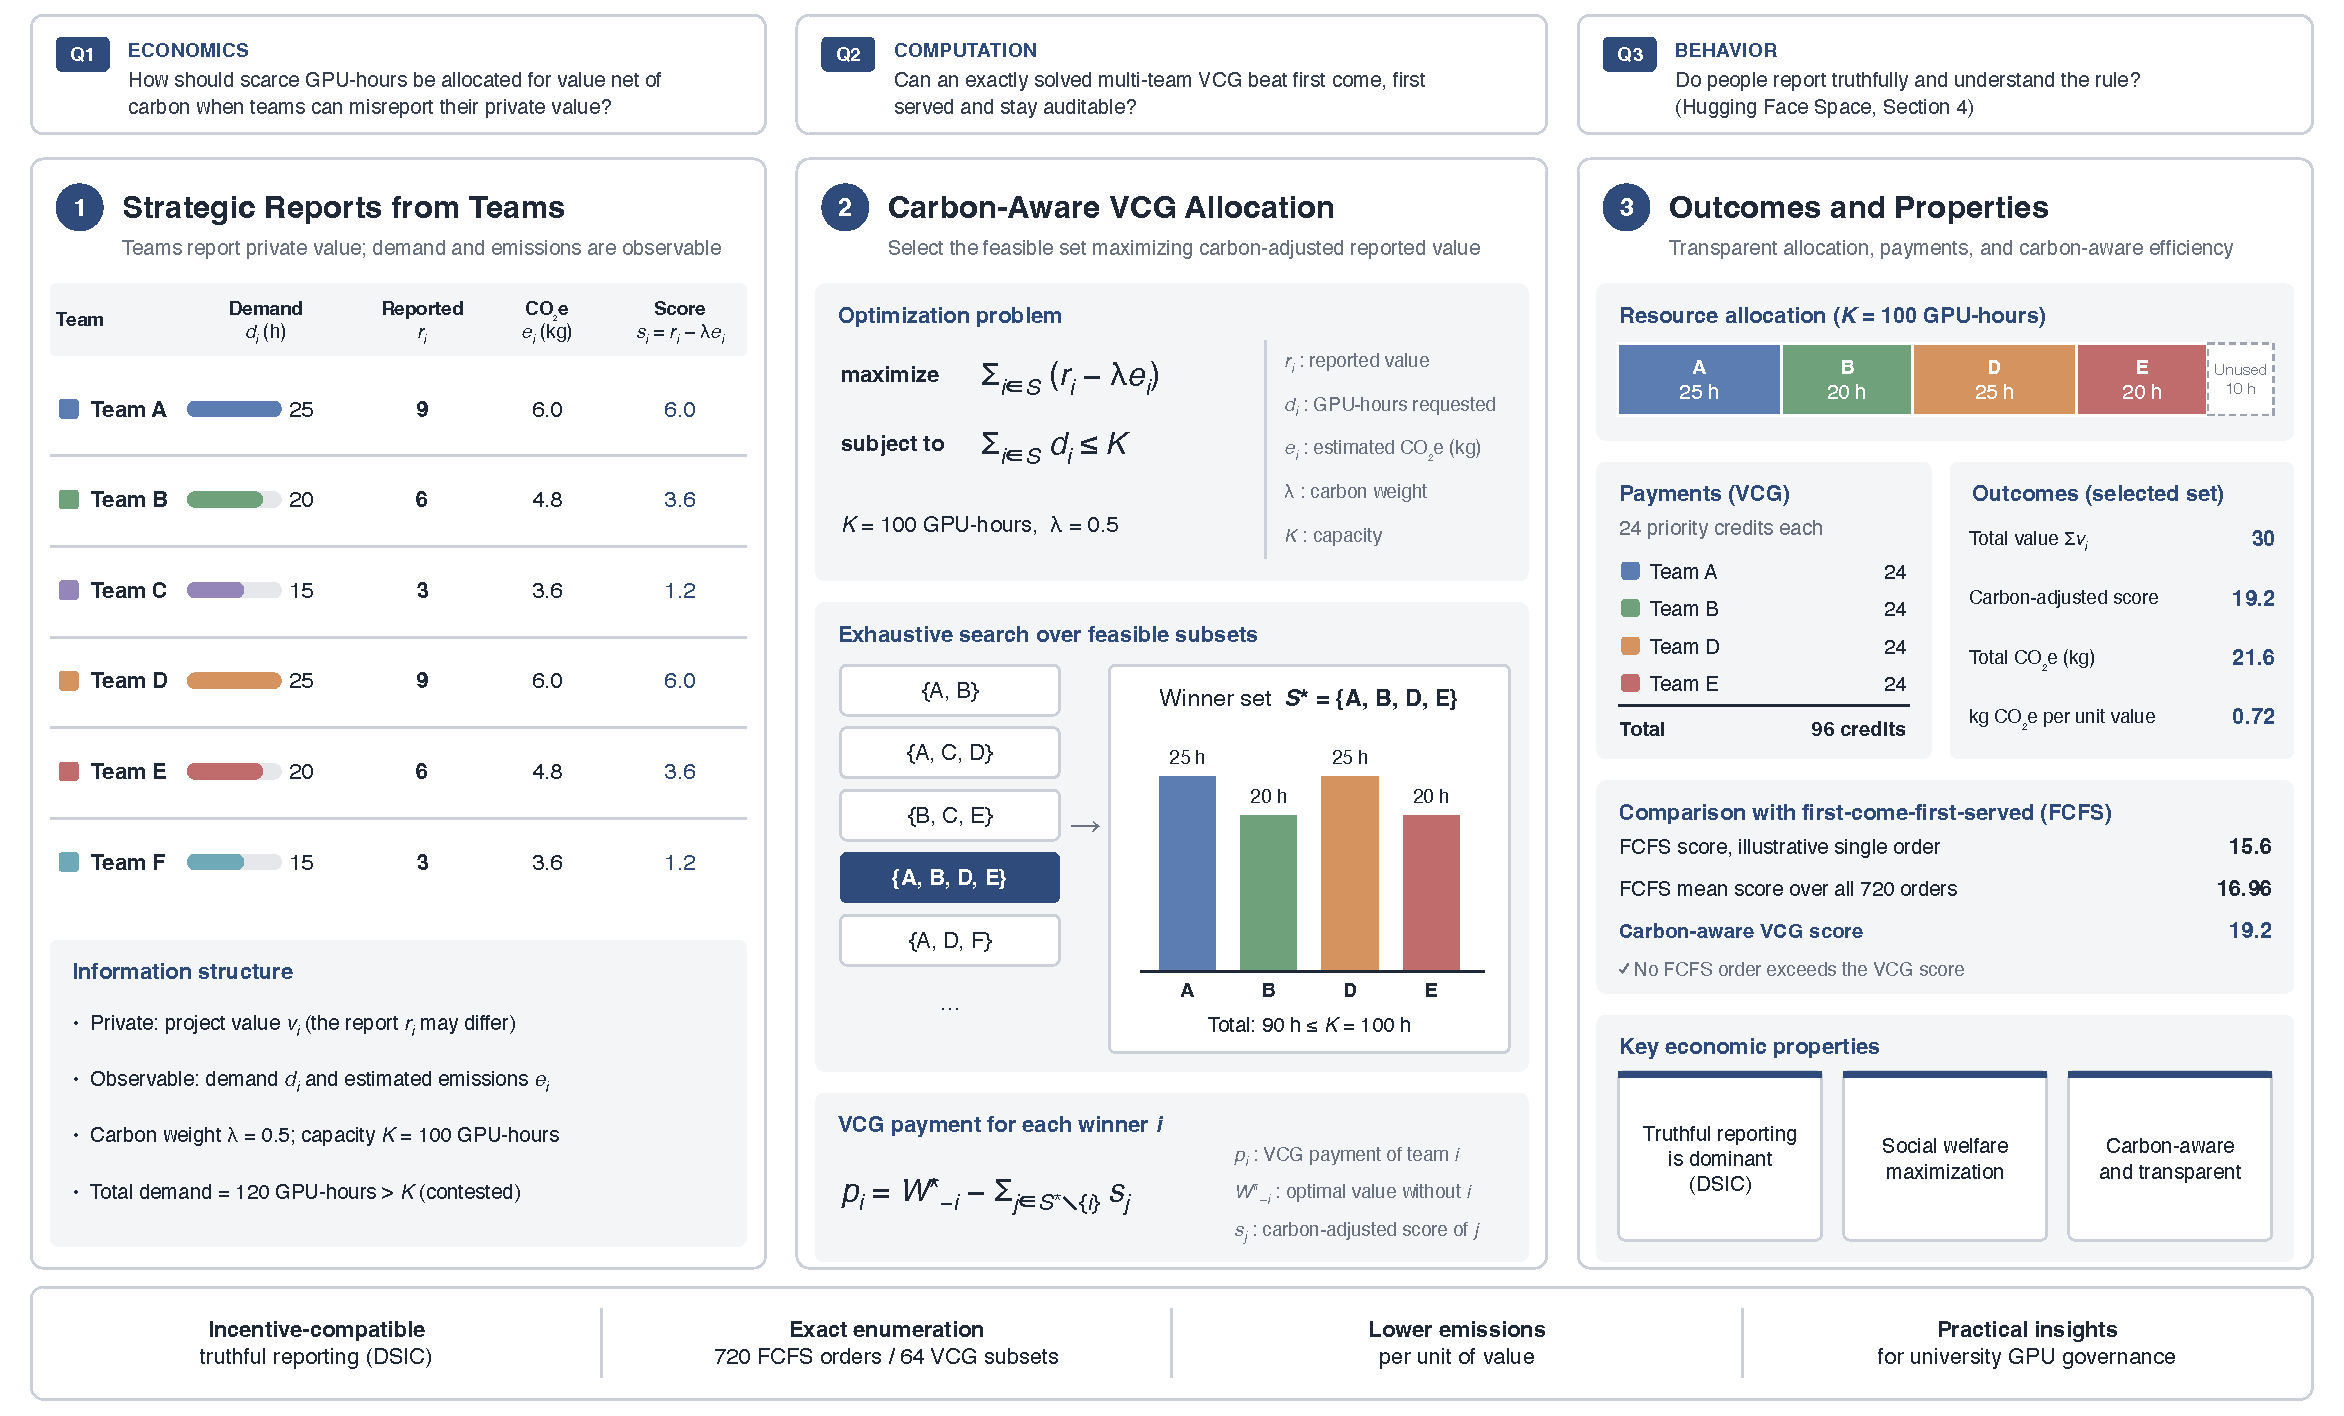
\includegraphics[
  width=\textwidth,
  keepaspectratio
]{figures/teaser_figure.pdf}
\caption{
Carbon-aware allocation of 100 shared GPU-hours across six project teams.
The top row states the three research questions; panels 1--2 give the strategic model (Q1), panel 3 its exact computation (Q2), and the behavioral question (Q3) is tested in the Hugging Face Space.
We compare random-order FCFS with a VCG mechanism that selects the feasible team set
maximizing reported project value minus a published carbon penalty and charges externality
payments.
}
\label{fig:teaser}
\end{teaserfigure}
\maketitle\raggedbottom\coursemeta

% Marker for text the team must still replace before submission. Search the source for \needchange.
\providecommand{\needchange}[1]{\textcolor{red}{\textbf{[NEED TO CHANGE: #1]}}}

\section{Three connected research questions and verified gap}

\noindent
Organizations increasingly face scarce GPU capacity as AI workloads grow. First-come-first-served allocation ignores project value and urgency, potentially misallocating scarce compute and leaving carbon costs unaccounted for.

\vspace{3pt}

\noindent
The closest work is Zachariadis et al.'s FAIR-Compute report~\cite{fair_compute2026}. Its method is a trace-driven simulation: it replays a public academic workload (Purdue Anvil, about 20.9 million jobs) under FIFO, Slurm-style priority, a tuned multi-objective priority, and an offline optimization benchmark. Its evidence is that online, value-blind rules recover only about 65\% of the available scientific value (1552--1612 of 2388 units; their Section~5.4), so roughly a third is lost. It also marks the two gaps we address: it does not quantify carbon (Section~3.6), and it warns that self-declared value will be exaggerated (Section~4.2) while leaving mechanisms under which truthful reporting is optimal to future work (Section~7). We build that missing piece. We trade their trace-level scale for a six-team instance that is solved exactly, so the allocation, the payments, and the truthfulness claim can each be re-checked by a reader.

\vspace{3pt}

\noindent
\textbf{Q1---Economics:} How should an institution allocate scarce GPU-hours to maximize project value net of carbon cost, when teams privately know their own value and can misreport it?\par
\textbf{Q2---Computation:} Can an exactly-solvable multi-team VCG mechanism allocate more efficiently than first-come-first-served, while staying auditable?\par
\textbf{Q3---Behavior:} Do participants report values close to the truthful benchmark, or does behavior deviate---and do their predictions and reflections show understanding of the rule?

\vspace{3pt}

\noindent
Together: can a transparent, carbon-aware rule replace arrival order, and does its advantage survive behavioral and computational limits? Figure~\ref{fig:teaser} states the three questions in its top row and traces the model (Q1) and its exact computation (Q2) below them; the behavioral test (Q3) is described in Section 4.

\section{Answer to Q1: incentives and strategic model}

\noindent
\textbf{Hypothesis.} An incentive-compatible, carbon-aware mechanism increases realized value and reduces emissions per unit of value, without misreporting.

\vspace{3pt}

\noindent
\textbf{Model.} Six teams $i\in\{A,\dots,F\}$ compete for $K=100$ GPU-hours. Each privately knows value $v_i \in \{3,6,9\}$; demand $d_i$ is observable, emissions $e_i=0.24d_i$ kg CO$_2$e, carbon weight $\lambda=0.5$ (stated parameters, not empirical estimates). Teams simultaneously submit one report $r_i$ (static, incomplete information).

\vspace{3pt}

\noindent
\textbf{Allocation and payment.} Score $s_i=r_i-\lambda e_i$; select feasible $S^*$ maximizing $\sum_{i\in S}s_i$ s.t. $\sum_{i\in S}d_i\le K$ (demand enters only as the constraint). Each winner pays the Clarke--Groves externality $p_i = W_{-i}^* - \sum_{j\in S^*\setminus\{i\}}s_j$~\cite{clarke1971,groves1973} (Appendix~A); utility is $u_i=v_i-\lambda e_i-p_i$ if selected, else 0.

\vspace{3pt}

\noindent
\textbf{Intuition.} The payment $p_i$ is the score the other teams lose because $i$ is selected, and it does not depend on $r_i$. Substituting it gives $u_i = (\text{true total score of } S^*) - W_{-i}^*$; the second term is fixed, so a team can raise its utility only by letting the rule pick the truly best group, which is what a truthful report does. A report therefore matters only through whether it crosses the team's selection boundary. Team C ($v_C=3$) is selected once $r_C\ge 4.2$, and every report above that boundary pays the same 2.4 and yields $u_C=-1.2$: overreporting more never costs more, it only buys a seat that is worth less than its price (Appendix~F.1).

\vspace{3pt}

\noindent
\textbf{Solution concept.} Truthful reporting $r_i=v_i$ is dominant---stronger than Nash/Bayesian Nash equilibrium~\cite{nash1950,harsanyi1968}---holding only because each team bears its own carbon penalty in $u_i$ (else the optimum shifts to $r_i=v_i+\lambda e_i$) and credits carry real future cost; verified numerically over $[0,10]$ for every team and for every carbon weight $\lambda\in\{0,0.1,\dots,1\}$ (Appendix~A.2). A reduced $2\times2$ payoff matrix for Teams C and E is in Appendix~A.1 (Table~\ref{tab:matrix}).

\vspace{3pt}

\noindent
\textbf{Three lenses.} Game theory yields the dominant-strategy prediction. Social choice frames the objective as value net of carbon under capacity and surfaces two trade-offs: efficiency against access (VCG serves 4 teams against an FCFS mean of 4.93), and truthfulness against budget balance (the 96 credits go to the organization rather than back to teams; returning them would in general break truthfulness~\cite{greenlaffont1977}, so they are the price of a dominant strategy). Mechanism design specifies the report space, the rules, and the verified tests (Appendix~C).

\section{Answer to Q2: computation, auction comparison, and artifacts}

\noindent
\textbf{Inputs.} Six teams (A--F): demands $(25,20,15,25,20,15)$, values $(9,6,3,9,6,3)$. FCFS is evaluated over all 720 arrival orders; VCG enumerates all 64 feasible subsets and re-solves per winner for payments (Appendix~A.1--A.2).

\textbf{Result.} VCG selects $\{A,B,D,E\}$ (score 19.2)---no FCFS order of 720 exceeds it (range 15.6–19.2; mean 16.96). Emissions per value fall from 0.81--0.84 to 0.72 kg CO$_2$e. One verified synthetic instance, not general evidence (Appendix~A, GitHub).

\vspace{3pt}

\noindent
\textbf{Parameter change.} Sweeping $\lambda$ from 0 to 1 in steps of 0.1 changes payoffs but not strategy. The selected group is $\{A,B,D,E\}$ for every $\lambda\in[0.1,1]$. The payment per winner falls from 5.28 ($\lambda=0.1$) to 2.4 ($\lambda=0.5$) and to 0 (from $\lambda=0.9$), because the low-value teams stop competing for a seat; the utility of A and D is 3.12, 3.6, and 3.0 at $\lambda=0.1, 0.5, 1$. Truthful reporting is optimal at all eleven values. $\lambda$ is therefore a policy weight on carbon, not an incentive parameter, and it cannot be chosen by maximizing project value, since on value alone $\lambda=0$ always wins. A second change splits capacity into two GPU types (H100, 50 h at 0.24 kg; A100, 50 h at 0.14 kg): the same four teams win, the two largest jobs move to the cleaner pool, emissions fall from 21.6 to 16.6 kg, and truthful reporting stays optimal (Appendix~A.2).

\vspace{3pt}

\noindent
\textbf{Analogy boundary.} The auction analogy holds only in part. Payments are non-transferable priority credits rather than money, so the dominant-strategy result needs credits to carry a real future opportunity cost, which the code cannot verify. True values are never observed: allocation and payment use reports only. And unlike a single-item auction, several teams win under a capacity (knapsack) constraint that is solved by exact search over 64 groups; only with one slot and $\lambda=0$ does the rule reduce to a Vickrey second-price auction~\cite{vickrey1961}, a case our code reproduces (the winner pays the second-highest value).

\vspace{3pt}

\noindent
\textbf{Artifacts.} GitHub: \GitHubLink{} (commit \texttt{8a656a4}). Notebook: \NotebookLink. Hugging Face: \HuggingFaceLink{} (Space commit \texttt{ad5604b}). A0 poster: \texttt{PS2-FP05-TeamA-A0-Poster.pdf}.

\section{Answer to Q3: behavior and interdisciplinary integration}

\noindent
\textbf{Rational benchmark.} Section~2 establishes $r_i=v_i$ as dominant under VCG; FCFS has no reporting decision at all.

\vspace{3pt}

\noindent
\textbf{Behavioral mechanism and competing explanation.} Laboratory second-price auctions show persistent overbidding even though truthful bidding is dominant~\cite{kagel1987}. Two explanations predict the same overreport in our setting. (i)~\emph{Comprehension:} a sealed-bid VCG rule is not obviously strategy-proof, so players may not see that the truth is optimal~\cite{li2017}. (ii)~\emph{Preference:} players understand the rule but value winning itself~\cite{cooperfang2008}.

\vspace{3pt}

\noindent
\textbf{Computed consequences of each behavior.} The model shows what each deviation would cost; these rows are computed, not observed (rivals truthful, $\lambda=0.5$).

{\footnotesize
\begin{tabularx}{\columnwidth}{@{}p{2.25cm}p{1.45cm}Y@{}}\toprule
\textbf{Behavior} & \textbf{Own utility} & \textbf{Effect on other teams}\\\midrule
Truthful (all) & A,D 3.6; B,E 1.2; C,F 0 & baseline\\
A overreports, $9\to10$ & 3.6 (same) & none: A already holds a seat and its price is unchanged\\
C overreports, $3\to4.5$ & $0\to-1.2$ & E loses its seat; B falls to 0; A, D fall to 2.4\\
B underreports, $6\to4$ & $1.2\to0$ & B loses its seat; C and F enter\\\bottomrule
\end{tabularx}}

\vspace{3pt}

\noindent
A deviation in either direction never helps the deviating team, but an overreport that crosses the boundary also harms others: the rule guarantees that the liar does not gain, not that bystanders are protected.

\vspace{3pt}

\noindent
\textbf{Observed evidence (exploratory).} We recorded $n=5$ completed plays of the Space (\texttt{hf-space/plays.csv}), played by the three authors on October~3, 2026. Each player held a private value, chose a request and a report, and predicted the outcome before seeing it; the five rivals were simulated and truthful, and stakes were hypothetical.

{\footnotesize
\begin{tabularx}{\columnwidth}{@{}Ycc@{}}\toprule
\textbf{Measure} & \textbf{Benchmark} & \textbf{Observed}\\\midrule
Truthful reports ($r_i=v_i$) & 5/5 & 2/5\\
Mean $|r_i-v_i|$ & 0 & 1.8\\
Overreports / underreports & 0 / 0 & 3 / 0\\
Selection predicted correctly & --- & 3/5\\
Overreport with a wrong prediction & 0 & 1\\
Overreport with a correct prediction & 0 & 2\\
Plays in which a misreport raised utility & 0 & 0\\\bottomrule
\end{tabularx}}

\vspace{3pt}

\noindent
\emph{Agreement.} The payoff prediction held in every play: no overreport raised the player's utility. Two overreports left utility unchanged, and one bought a seat that cost 36 credits and was worth nothing net of carbon ($u=-3.6$ against 0 for the truth). \emph{Gap.} The behavioral prediction did not hold: three of five players overreported (by 4, 4, and 1), although the report field starts at the true value. Both wrong predictions were pessimistic (``left out'' when the team was selected). \emph{Consequence.} We retain the dominant-strategy result as a statement about payoffs and qualify the assumption that players see it: truthful reporting was optimal but not typical. The written reflections were left blank in all five plays. Asked afterwards, the players gave two reasons for overreporting: wanting to be selected, and misunderstanding the rule. These match explanations~(ii) and~(i), but they are recollections given after the result was known and were not recorded per play, so we do not assign them to individual plays. One further observation is consistent with explanation~(i): a symposium reviewer who had read the rule asked whether truthful reporting is optimal with and without the carbon charge (Appendix~D). These are five self-plays by the authors, who know the rule, against simulated rivals; they are exploratory and support no population claim. These observations motivate a larger classroom sample with written reflections, but they do not predict how often other participants will misreport.

\vspace{3pt}

\noindent
\textbf{Interaction.} Users play one team through both FCFS and VCG stages, predicting their own selection before seeing the result, then inspect the ranking, payments, and utility (full mechanics in Appendix~F.1). All evidence is exploratory, with participant count and conditions reported.

\vspace{3pt}

\noindent
\textbf{Discriminating observation.} The prediction step separates the two explanations. An overreport with a \emph{wrong} selection prediction points to comprehension~(i) and would lead us to revise the interface (show the what-if curve before the report). An overreport with a \emph{correct} prediction and a reflection about wanting to win points to preference~(ii) and would lead us to revise the model (add a value of winning to $u_i$). Neither supports a causal claim. The first five plays contain one case of the first kind and two overreports with a correct prediction but no written reflection, so the next step is the interface revision, which also requires the reflection before the result line can be copied (planned).

\section{Advanced development, real-world impact, and roadmap}

\noindent
This proposal builds on two Nobel-recognized foundations: Vickrey's theory of incentives under asymmetric information~\cite{vickrey1961,nobel1996} and Hurwicz--Maskin--Myerson's mechanism design theory~\cite{nobel2007}---agents can be motivated to reveal the truth without verifying private information. The model is specified enough to support a transparent pilot design, but its parameters remain classroom assumptions. Integrating incentive-compatible allocation, an explicit carbon objective, and exploratory behavioral evidence addresses the two gaps left by Section~1's closest prior work.

\vspace{3pt}

\noindent
The concrete case is a shared university GPU cluster. Teams benefit from allocation reflecting true value; administrators gain an auditable record; the public bears the carbon cost regardless of who benefits. Honest reporting is incentivized, but truthfulness relative to a team's actual beliefs is not independently verifiable. The carbon weight $\lambda$ is the institution's choice, for example an internal carbon price converted into value units; our sweep shows the allocation is stable for $\lambda\in[0.1,1]$, while a weight that is too heavy stops research (only A and D are served above $\lambda=1.25$, and no team above $\lambda=1.5$). Academic adoption would accept a transparent pilot; industry would demand robustness at hundreds of teams; public institutions would require an independently re-runnable audit. Next test: a pilot comparing self-reported value against ex-post outcomes at a scale where exact solving is no longer tractable. Planned voting bridge: a variant in which teams rank the projects and the rule aggregates the rankings (plurality against Borda), to compare manipulation under voting with misreporting under VCG; this is planned work, not a result.

\vspace{3pt}

\begin{table}[h]
\caption{From foundations to a collaborative interdisciplinary contribution.}
\begin{tabularx}{\columnwidth}{@{}p{1.6cm}Y@{}}
\toprule
\textbf{Horizon}&\textbf{Milestone and evidence}\\
\midrule
Foundation&Vickrey~\cite{nobel1996} and Hurwicz--Maskin--Myerson~\cite{nobel2007}: incentive-compatible allocation without verifying private information.\\
PS2&Six-team carbon-aware VCG mechanism, exactly solved and verified against a random-order first-come-first-served baseline over all 720 arrival orders (Appendix~A).\\
Symposium&Poster on institutional GPU governance (Sept.~28). Peer challenges: carbon-weight calibration, a single GPU type, missing play data, and whether truth stays optimal with a carbon charge. Response: a $\lambda$ sweep, a two-GPU-pool extension, computed behavior scenarios, and five recorded self-plays (Appendix~D).\\
Next study&A rerun of the FCFS--VCG comparison over randomly drawn values and requests, then a pilot comparing self-reported value against independent, ex-post project outcomes at a scale where exact solving is no longer tractable.\\
2056&Auditable mechanism-design tool adopted by a real institution for actual, not simulated, compute governance.\\
\bottomrule
\end{tabularx}
\end{table}

\vspace{3pt}

\noindent
\noindent\textbf{Expected 2056 Nobel Prize and Turing Award contribution statement.}
By 2056, we aim to be recognized for an efficient, publicly auditable governance framework for scarce shared infrastructure, integrating an incentive-compatible mechanism, verifiable computation, and behavioral evidence on truthful reporting. Progress moves from this six-team simulation to a real institutional pilot, correctable through a public, re-runnable audit log.

\subsection*{Open Science Statement}
GitHub (\url{https://github.com/dku-comsci-econ206-Autumn2026/FP05-PS2-Team-A}) contains the FCFS/VCG code, tests, and outputs, including the carbon-weight sweep (\texttt{lambda\_sweep.csv}); a self-contained Colab notebook (\url{https://colab.research.google.com/drive/14eo8a2HWUbbBtv-m-ia4xRiL4V6Iwtun}) that also holds the two-GPU-pool extension; a Hugging Face Space (\url{https://huggingface.co/spaces/dku-comsci-econ206-2026/PS2_Team_A}, commit \texttt{ad5604b}); README with run instructions. Inputs are synthetic ($d_i\in\{15,20,25\}$, $v_i\in\{3,6,9\}$; the Space allows wider ranges), clearly labeled. Review-ready results come from commit \texttt{d93fc2e}; final results from commit \texttt{8a656a4}. Limitation: exact enumeration does not scale past small team counts.

\subsection*{Statement of Contribution to the UN's SDGs}
Connects to SDG~13 (carbon priced into allocation) and SDG~9 (auditable infrastructure rule). Audience: compute administrators and research teams; minimal access needs. Indicator: emissions per unit of allocated value. Possible unintended effect: urgency inflation beyond the report's resolution, or $\lambda$ disadvantaging compute-heavy research. Intended mechanism only---no adoption has occurred.

\clearpage\nobalance
\section*{Author Notes}
\subsection*{Acknowledgements}
\textbf{Course instructor: Professor Luyao Zhang.} We thank the symposium reviewers whose comments changed this version (Appendix~D): Yiqiao Liu (FP10) and Aaron Wang (FP8), whose questions about how the carbon weight is chosen led to the $\lambda$ sweep; Zimu Zhou (FP11), whose single-GPU-type concern led to the two-pool extension; Xinrong Sun (FP9), whose question about truthful reporting with and without the carbon charge led to the intuition paragraph in Section~2; Yongzhuo Wu (FP1), who pointed out the missing play data; and Zijie Wang (FP7), whose comment on figure clarity led to the vector version of Figure~\ref{fig:teaser} and its research-question row. \needchange{add the reviewers of Mustafa and Temur.} Feedback does not imply coauthorship. We acknowledge the software this work relies on: Python and its standard library, Jupyter and Google Colab, matplotlib, Hugging Face Spaces, and diagrams.net (draw.io) for Figure~\ref{fig:teaser}. Generative AI assistance is disclosed in Appendix~A.3. The authors remain responsible for the proposal and remaining errors.

\subsection*{Team and individual contributions}

\textbf{Joint contribution.} Our team studies how an organization can allocate scarce shared GPU-hours when teams privately know their project value but GPU demand and estimated emissions are observable. We compare a random-order FCFS baseline, computed over all 720 arrival orders, with a transparent carbon-aware VCG mechanism that selects a feasible group of teams under a 100 GPU-hour capacity limit. Temur supplies the formal model, exact computation, and reproducibility checks; Mustafa develops the social-choice, governance, and real-world-impact argument; Gihun develops the interactive explanation, artifact interface, and poster layout. These parts form one research argument: a stated allocation rule is useful only when its strategic assumptions, computational results, public explanation, and limits can be inspected together. All three members will jointly review the final paper and artifacts for consistency.

\textbf{Temur Akhtamjonov.} I designed the six-team GPU-allocation model, implemented the FCFS baseline and the exhaustive VCG solver, and verified the reported allocation, capacity, score, emissions, and payment outputs. My key decision was to model the setting as a multi-winner direct mechanism rather than a one-winner auction. My evidence is the GitHub simulation, runnable Colab notebook, and saved output files. This work provides the formal and computational basis for the paper, Hugging Face interaction, and poster. My next responsibility is to check that all three artifacts use the same parameters, allocation rule, and reported results. \needchange{Temur: state what you did after the symposium and your next responsibility.}

\textbf{Mustafa Ayub Khan.} I developed the social-choice and mechanism-design framing: writing the literature review identifying FAIR-Compute as the closest prior work and the specific gap it leaves open---an incentive-compatible, carbon-aware allocation rule it names as future work but does not build---and drafting the real-world-impact case distinguishing academic, industry, and public-institution evidence standards for adoption. My key decision was identifying that an early fixed-price allocation formula (score proportional to GPU-hours alone) had silently dropped private project value from the mechanism, and proposing the corrected selection rule $s_i = r_i - \lambda e_i$, which restores private value as the basis for selection and keeps demand as only a capacity constraint---the formula the team's VCG mechanism is built on. I also treated auditability of execution, not verification of private values, as the honest limit of this mechanism's transparency. My evidence is Sections~1, 2, and~5, the Open Science and SDG statements, and Table~1's roadmap. I independently re-derived Temur's FCFS and VCG allocation numbers by hand against the stated $v_i$, $d_i$, and $\lambda=0.5$, confirming the reported subsets, scores, and total payment of 9.6 score units (96 priority credits). This argument depends on Temur's simulation producing the value/carbon trade-off Section~5 describes, and feeds the poster's real-world-case panel and Gihun's audit-trail framing in the Hugging Face interface. My next responsibility is to check symposium feedback against Section~5's adoption-evidence claims and revise the real-world case accordingly. \needchange{Mustafa: state what you did after the symposium and your next responsibility.}

\textbf{Gihun Lee.} I built the public-facing allocation audit and the reproducibility interface: the Hugging Face Space, the GitHub README, the self-contained Colab notebook structure, Figure~\ref{fig:teaser}, and the poster layout. My key decision was to make the stated rule checkable against its visible execution: in the Space a player holds a private true value, reports separately, predicts their own selection, and then sees the score ranking, winning group, VCG payments, utility, and a what-if curve of utility against every report. While building this audit, I found that the original utility $v_i-p_i$ contradicted the paper's dominant-strategy claim, because under it a team gains by reporting $v_i+\lambda e_i$. I proposed $u_i=v_i-\lambda e_i-p_i$, added a truthfulness sweep, and replaced the single FCFS queue with all 720 arrival orders. My evidence is the Space, the \texttt{colab/} folder (tests, outputs, notebook), and the README. I verified that the unit tests pass, that the notebook runs 9/9 checks in a clean folder without the repository, that the browser port matches the Python code on 300 random games, and that \texttt{run\_simulation.py} reproduces the committed outputs. This work turns Temur's computation and Mustafa's framing into an interface a non-specialist can inspect. \emph{Revision after the symposium.} I recorded six peer reviews of the project on my response form and made the following revisions (decisions in Appendix~D, change list in Appendix~F.3).
(1)~\emph{Carbon weight} (Yiqiao Liu, Aaron Wang): I swept $\lambda$ from 0 to 1 and reported both what it changes (prices, payoffs, selection boundaries) and what it cannot change (the best strategy). My key decision was to treat $\lambda$ as a policy weight rather than a parameter to optimize, because on project value alone $\lambda=0$ always wins. Output: the notebook's sweep cells, \texttt{run\_simulation.py}, and \texttt{lambda\_sweep.csv}; Section~3 and Appendix~A.2.
(2)~\emph{GPU types} (Zimu Zhou): I added a two-pool extension (H100 and A100) in which the rule also chooses each team's pool, and recorded its limit, that it ignores speed differences. Output: notebook, Appendix~A.2--A.3.
(3)~\emph{Truthfulness with and without the carbon charge} (Xinrong Sun): I added the payment intuition to Section~2 and the exact selection boundary for Team C ($r_C\ge4.2$), and I stated the analogy boundary in Section~3 with a unit test showing that one slot with $\lambda=0$ is a second-price auction.
(4)~\emph{Missing play data} (Yongzhuo Wu): I added the behavioral mechanism, the competing explanation, and the computed consequence of each behavior type to Section~4. My key decision here was to label these rows as computed and to report the five recorded plays separately as observed, so that simulated behavior is never presented as observed behavior.
(5)~\emph{Figure clarity} (Zijie Wang): I re-exported Figure~\ref{fig:teaser} as a vector PDF and added a top row that states the three research questions, so the figure itself shows how Q1--Q3 connect to the panels. Output: \texttt{figures/teaser\_figure.pdf}, \texttt{.svg}, \texttt{.png}, and the editable \texttt{.drawio}.
(6)~\emph{Other revisions}: the method-by-method comparison with the closest work in Section~1, the budget-balance trade-off in Section~2 and Appendix~C, the corrected $\lambda$ statement in Appendix~C, the README, and Appendices~D, E, and F.3.
Verification: I reran everything on October 3, 2026: 7 unit tests pass, the notebook passes 9/9 checks in an empty folder, and the committed v1 outputs are reproduced without a diff. The rerun also corrected two of my own first-draft review responses: payments fall rather than rise as $\lambda$ increases, and the price is unchanged by a team's own report, not by the carbon charge. Connection: these revisions use Temur's model code unchanged and extend Mustafa's social-choice argument with the access and budget-balance trade-offs. I also recorded five completed plays of the Space, exported them as an anonymous table (\texttt{hf-space/plays.csv}), and compared them with the benchmark in Section~4: no misreport raised utility, but three of five players overreported. I added a notice to the Space that states what the class form collects. The five plays are self-plays by the three authors on October~3, 2026. My next responsibility is to collect more plays with the written reflection filled in, show the what-if curve before the report, and keep the poster, paper, and artifacts at parity.

\bibliographystyle{ACM-Reference-Format}\bibliography{references}
\appendix
\section{Technical details and reproducibility}

\subsection{Model inputs and rules}

This project uses one fixed synthetic classroom example with six teams and a capacity of $K=100$ GPU-hours. Table~\ref{tab:inputs} gives the inputs. Values are private to teams but are reported truthfully in the baseline computation. GPU-hour demand is observable. Estimated emissions use the stated classroom assumption $e_i=0.24d_i$ kg CO$_2$e. The announced carbon weight is $\lambda=0.5$, so each reported score is
\[
s_i=r_i-\lambda e_i=r_i-0.5(0.24d_i).
\]

\begin{table}[h]
\centering
\caption{Fixed synthetic inputs used in the fresh run.}
\label{tab:inputs}
\begin{tabular}{lrrr}
\toprule
Team & GPU-hours $d_i$ & Value $v_i$ & Emissions $e_i$ \\
\midrule
A & 25 & 9 & 6.0 \\
B & 20 & 6 & 4.8 \\
C & 15 & 3 & 3.6 \\
D & 25 & 9 & 6.0 \\
E & 20 & 6 & 4.8 \\
F & 15 & 3 & 3.6 \\
\bottomrule
\end{tabular}
\end{table}

The FCFS baseline uses a random arrival order. Each team receives its full request only when the request fits in the remaining capacity. We compute all $6!=720$ orders exactly and report A, B, E, C, D, F as one illustrative draw. The proposed mechanism is a simultaneous-report, multi-winner VCG direct mechanism. It chooses the feasible subset $S$ that maximizes total reported score:
\[
\max_{S \subseteq N}\sum_{i\in S}s_i
\quad \text{subject to} \quad
\sum_{i\in S}d_i\leq K.
\]
For each selected team $i$, the priority-credit payment is its reported-score externality:
\[
p_i=
\max_{S'\subseteq N\setminus\{i\}}\sum_{j\in S'}s_j
-
\sum_{j\in S\setminus\{i\}}s_j.
\]
One payment score unit equals 10 non-transferable priority credits in this classroom model. A selected team's utility is $u_i=v_i-\lambda e_i-p_i$, and an unselected team's utility is $0$. Each team bears its own carbon penalty; this is what makes truthful reporting dominant.

\textbf{Reduced payoff matrix.} The full game has six players and a continuum of reports, so it has no single matrix. Table~\ref{tab:matrix} is a labeled simplification: only Teams C and E choose, each between its truthful report and one deviation, while A, B, D, and F report truthfully. Every cell is computed by the same \texttt{vcg\_allocation} code (notebook cell ``Reduced payoff matrix'').

\begin{table}[h]
\centering
\caption{Reduced $2\times2$ game: utilities $(u_C,u_E)$ and the selected group.}
\label{tab:matrix}
\footnotesize
\begin{tabular}{lcc}
\toprule
 & E truthful ($r_E=6$) & E underreports ($r_E=4$) \\
\midrule
C truthful ($r_C=3$) & $(0,\;1.2)$, ABDE & $(0.8,\;0)$, ABCDF \\
C overreports ($r_C=4.5$) & $(-1.2,\;0)$, ABCDF & $(0.8,\;0)$, ABCDF \\
\bottomrule
\end{tabular}
\end{table}

For Team C, the truthful row is never worse than the overreport row ($0\ge-1.2$ and $0.8\ge0.8$). For Team E, the truthful column is never worse than the underreport column ($1.2\ge0$ and $0\ge0$). Truth is therefore weakly dominant for both, and (truthful, truthful) is the equilibrium of the reduced game, matching the dominant-strategy result of the full model. The lower-left cell also shows the externality: C's overreport removes the truthful Team E from the group.

\subsection{Exact algorithm and fresh-run record}

The implementation checks every possible subset of six teams.

\begin{enumerate}
\item Enumerate all $2^6=64$ subsets.
\item Remove a subset if its total requested GPU-hours exceed 100.
\item Compute total reported score for every remaining subset.
\item Select the subset with the largest score. Ties are broken publicly by first serving more teams and then using deterministic team order.
\item For each selected team, repeat the calculation without that team and compute its externality payment.
\item Truthfulness check: for each team, re-run steps 1--5 with its report set to $0,0.5,\dots,10$, holding the other teams fixed, and confirm that no report beats $r_i=v_i$.
\item Carbon-weight sweep: repeat steps 1--6 for $\lambda=0,0.1,\dots,1$.
\item Two-GPU-pool extension: choose who is served and on which pool (all $3^6=729$ assignments), then repeat steps 5--6.
\end{enumerate}

A fresh run of \texttt{python colab/run\_simulation.py} reproduces the saved summary, team-level, all-orders, truthfulness, and carbon-weight-sweep CSV outputs in the repository's \texttt{colab/outputs} folder. The same calculation is available in our self-contained Colab notebook (\NotebookLink).

The saved fresh-run comparison is:

\begin{center}
\small\setlength{\tabcolsep}{3pt}
\begin{tabularx}{\columnwidth}{@{}Yrrrr@{}}
\toprule
Rule & GPU-h & Value & CO$_2$e & Score \\
\midrule
FCFS (A,B,E,C,D,F) & 95 & 27 & 22.8 & 15.6 \\
FCFS, 720-order mean & 97.0 & 28.6 & 23.28 & 16.96 \\
VCG (A,B,D,E) & 90 & 30 & 21.6 & 19.2 \\
\bottomrule
\end{tabularx}
\end{center}

In the illustrative order, FCFS serves A, B, E, C, and F and leaves 5 GPU-hours unused. Across all 720 orders, the FCFS carbon-adjusted score ranges from 15.6 to 19.2, and no order exceeds VCG. VCG leaves 10 GPU-hours unused and collects 9.6 payment score units, equal to 96 priority credits (2.4 per winner). Utilities are 3.6 for A and D, 1.2 for B and E, and 0 for C and F. For every team, no report in $[0,10]$ yields higher utility than $r_i=v_i$. The notebook's final cell prints PASS for nine checks: allocation, capacity, value and score, payments, utilities, truthful optimality, the 720-order comparison, truthful optimality at every carbon weight, and the two-GPU-pool extension. A repository test confirms that the notebook's model code is identical to \texttt{colab/src/gpu\_allocation.py}.

\textbf{Carbon-weight sweep} (\texttt{colab/outputs/lambda\_sweep.csv}; demands, values, capacity, and algorithm fixed).

\begin{center}
\footnotesize\setlength{\tabcolsep}{3pt}
\begin{tabularx}{\columnwidth}{@{}rYrrrc@{}}
\toprule
$\lambda$ & Selected & Pay & $u_{A,D}$ & $u_{B,E}$ & Truth \\
\midrule
0.0 & A,B,C,D,F & 6.0$^{*}$ & 3.00 & 0.00 & yes \\
0.1 & A,B,D,E & 5.28 & 3.12 & 0.24 & yes \\
0.3 & A,B,D,E & 3.84 & 3.36 & 0.72 & yes \\
0.5 & A,B,D,E & 2.40 & 3.60 & 1.20 & yes \\
0.7 & A,B,D,E & 0.96 & 3.84 & 1.68 & yes \\
0.9 & A,B,D,E & 0.00 & 3.60 & 1.68 & yes \\
1.0 & A,B,D,E & 0.00 & 3.00 & 1.20 & yes \\
\bottomrule
\end{tabularx}
\end{center}
{\footnotesize Pay: payment per winner in score units. $^{*}$At $\lambda=0$, C and F pay 3.0. Truth: no report in $[0,10]$ beats $r_i=v_i$ for any team. The CSV holds all eleven values.}

\emph{What $\lambda$ changes.} It moves each team's selection boundary, the price, and the size of the payoff. At low $\lambda$ the low-value teams C and F still compete for a seat, so winners pay more (5.28 at $\lambda=0.1$). As $\lambda$ rises their scores turn negative, competition fades, and the price falls to 0 from $\lambda=0.9$; from that point a heavier own carbon charge $\lambda e_i$ lowers the winners' utility. Team C's selection boundary moves from $r_C\ge3.25$ ($\lambda=0.1$) to 4.2 ($\lambda=0.5$) and 4.8 ($\lambda=1$).
\emph{What $\lambda$ does not change.} Truthful reporting is optimal for every team at every $\lambda$ in the sweep, because a team's price never depends on its own report. $\lambda$ is a policy weight on carbon, not an incentive parameter. It also cannot be chosen by maximizing project value: on value alone, $\lambda=0$ always wins.
\emph{The change at $\lambda=0$.} Groups $\{A,B,C,D,F\}$ and $\{A,B,D,E\}$ tie on value (30). The public tie-break selects more teams; any $\lambda>0$ breaks the tie toward the group that uses fewer GPU-hours.
\emph{Beyond the sweep.} Above $\lambda=1.25$ only A and D are served, and above $\lambda=1.5$ no team is served.

\textbf{Two-GPU-pool extension} (notebook only). The 100 GPU-hours are split into an H100 pool (50 h, 0.24 kg CO$_2$e per GPU-hour, the baseline rate) and an A100 pool (50 h, 0.14 kg). A team runs entirely on one pool, and the score uses the assigned pool's rate.

\begin{center}
\footnotesize\setlength{\tabcolsep}{3pt}
\begin{tabularx}{\columnwidth}{@{}p{2.3cm}YY@{}}
\toprule
 & One pool & Two pools \\
\midrule
Selected & A, B, D, E & A, B, D, E \\
Placement & --- & A, D on A100; B, E on H100 \\
CO$_2$e (kg) & 21.6 & 16.6 ($-23\%$) \\
kg per unit value & 0.72 & 0.55 \\
Payments & 2.4 each & A, D 3.65; B, E 2.4 \\
Utilities & A, D 3.6; B, E 1.2 & unchanged \\
Truth optimal & yes & yes \\
\bottomrule
\end{tabularx}
\end{center}

The two largest jobs move to the cleaner pool. A and D pay more because, without A, other teams could use its clean A100 hours, so A's externality is larger. Utilities and selection boundaries are unchanged, and no report beats the truth: the Groves argument needs only that the best feasible outcome is found exactly, however many capacity constraints there are.

\subsection{Reproducibility, limits, and AI-use disclosure}

\textbf{Reproducibility.} The GitHub repository (\GitHubLink) contains the source code, tests, notebook, output files, and README instructions in \texttt{colab/}. The model, script, and tests use only the Python standard library. The notebook's utility plots use matplotlib, which Colab provides. Review-ready results come from commit \texttt{d93fc2e} (tag \texttt{ps2-review}); final results come from \needchange{final commit or tag}. Final rerun, October 3, 2026 (Python 3.14.7, macOS arm64): \texttt{run\_simulation.py} reproduces the committed outputs and writes \texttt{lambda\_sweep.csv}; 7 unit tests pass; the notebook passes 9/9 checks in an empty folder without the repository.

\textbf{Limits.} This is a small synthetic example, not a field deployment. The 0.24 kg CO$_2$e per GPU-hour rate, the carbon weight, the value tiers, and the 10-credit conversion are classroom assumptions. Exact enumeration will not remain practical as the number of teams becomes large. The model also cannot verify a team's true private value. The baseline has one GPU type; the two-pool extension assumes a job needs the same GPU-hours on either type, whereas an A100 is slower than an H100 in practice, so it is a structural check and not an emissions estimate. Truthful reporting is dominant only if priority credits carry a real future opportunity cost; the code checks the rule, not that condition. Human play is limited to five self-plays by the authors against simulated, truthful rivals with hypothetical stakes, and their written reflections are blank.

\textbf{AI-use disclosure.} The team used Claude Code (Claude Opus 5.5, Anthropic).
\emph{September 25--26, 2026.} Purpose: build the Hugging Face Space, restructure the README and the self-contained notebook, write the simulation code and unit tests, and draw Figure~\ref{fig:teaser}.
\emph{October 3, 2026.} Purpose: respond to the symposium reviews. Significant prompts: explain why a team cannot gain by overreporting; compare the review-ready draft with the grading guide; sweep $\lambda$ from 0 to 1; simulate two GPU types with different emission rates; draft the revision text. Accepted: the carbon-weight sweep and \texttt{lambda\_sweep.csv}, the two-GPU-pool notebook cells, two new unit tests, the README update, the intuition paragraph in Section~2, and drafts of Sections~3--4 and Appendices~A, D, E, and F.3. The assistant also corrected two of our draft review responses: payments fall rather than rise as $\lambda$ increases, and Team C's selection boundary is $r_C\ge4.2$. Rejected: full redesigns of Figure~\ref{fig:teaser}; we kept the original figure and accepted only a research-question row above it and a vector export. Human changes: \needchange{list the edits the authors made to the AI-drafted text.} Verification: every reported number is produced by repository code (7 unit tests; 9 notebook checks in a clean folder), and the closest-work statements in Section~1 were checked against the FAIR-Compute text, and the authors confirmed the cited section numbers and the four added references. The human authors are responsible for every claim, citation, and computation.

\section{Cumulative Intellectual Development}
\textbf{Mustafa Ayub Khan -- prior development.} In PS1, Mustafa studied whether greater observability changes voluntary disclosure in a public-goods setting. Following Professor Zhang's September 7 feedback, he narrowed the claim and proposed a 2-by-2 design to distinguish genuine behavioral change from merely visible performance. This led to one bounded lesson for PS2: making a rule and its execution observable can improve accountability, but it cannot prove that a participant's private motive or value report is true. In the GPU-allocation project, this lesson appears in the published allocation rule, parameters, code, payments, and allocation log.

\textbf{Gihun Lee -- prior development.} In PS1, Gihun developed a transparent way to compare heterogeneous AI subscription plans using workload-specific measures, reproducible computation, sensitivity checks, and a public-facing interaction. Feedback on trustworthiness led him to avoid one opaque summary number and instead show the underlying components and assumptions. In PS2, this becomes the Hugging Face allocation audit: users can compare FCFS and the VCG mechanism, inspect the reported inputs and outcomes, see the stated assumptions behind the result, and check with a what-if curve whether truthful reporting maximizes their own utility. The same lesson shaped the revision after the September 28 symposium: reviewers asked why $\lambda=0.5$ and whether one GPU type is enough, so instead of defending one headline number Gihun showed the components. The carbon-weight sweep reports what $\lambda$ changes (prices, payoffs, selection boundaries) and what it does not (the best strategy); the two-GPU-pool extension reports which results survive a second capacity constraint; and Figure~\ref{fig:teaser} now states the three research questions above the panels. Affected locations: Sections~2--4, Appendix~A.2, and Figure~\ref{fig:teaser}.

\textbf{Temur Akhtamjonov -- development into the shared model.} Temur's earlier work on a commitment-bond trust game used a clear benchmark, a controlled rule change, and verified computational outputs. In PS2, he transfers this methodological approach to a new shared setting: hold the six-team GPU environment fixed, compare FCFS with carbon-aware VCG, enumerate all feasible allocations exactly, and report the resulting allocation and payments.

\textbf{Intellectual consequence.} PS2 is a new joint project, not a continuation of one PS1 topic. Its common development is methodological: each prior project emphasized a clear rule, visible assumptions, reproducible computation, and careful limits on what observed behavior can establish. Our shared contribution applies these principles to a transparent, carbon-aware allocation of scarce organizational GPU-hours.

\section{Open-source and three-lens inspiration}
\textbf{Sources and tools.} PS1 source records are preserved in each author's PS1 submission; the tools below are those used in PS2.

{\footnotesize
\begin{tabularx}{\columnwidth}{@{}p{1.6cm}Y@{}}\toprule
\textbf{Source / tool}&\textbf{URL, license, version; capability; limitation; design consequence}\\\midrule
Python standard library&\url{https://www.python.org}; PSF License; 3.13--3.14 locally, Colab runtime. Exact subset enumeration and permutations with no installs. Exponential in team count. Kept the model dependency-free so anyone can re-run it.\\
Jupyter / Google Colab&\url{https://jupyter.org} (BSD-3), \url{https://colab.research.google.com} (Google service terms). Runnable notebook with saved outputs. Hosted runtime can change over time. Notebook made self-contained, with a test that it matches \texttt{src/}.\\
matplotlib&\url{https://matplotlib.org}; matplotlib license (PSF-based); 3.11. Utility-versus-report plots. Plots only. Used only outside the model code.\\
Hugging Face Spaces (static)&\url{https://huggingface.co/docs/hub/spaces-sdks-static}; hosted service. Serves an HTML/CSS/JS page with no server. Cannot store responses. Evidence is collected by participants copying a result line rather than by server logging.\\
Claude Code&\url{https://claude.com/claude-code}; Anthropic terms; Claude Opus 5.5, Sept.--Oct.~2026. Coding and drafting assistant. Can err, so all outputs were tested. See Appendix~A.3.\\\bottomrule
\end{tabularx}}

\textbf{How each lens altered the shared model.}
\emph{Game theory:} framing the setting as a static game with incomplete information made $r_i=v_i$ the benchmark to test. Testing it (observation) showed that the original utility $v_i-p_i$ rewards overreporting by $\lambda e_i$, so the utility now includes each team's own carbon penalty.
\emph{Social choice:} stating the objective as value net of carbon under capacity exposed the efficiency--access trade-off. VCG serves 4 teams against an FCFS mean of 4.93 (observation). We interpret this as a real cost of the rule rather than a flaw to hide. A second incompatibility is budget balance: the 96 credits collected go to the organization, not back to the teams, because redistributing them would in general break truthfulness~\cite{greenlaffont1977}.
\emph{Mechanism design:} it fixed the report space, allocation, payment, and public tie-break, and it turned FCFS from one arbitrary queue into all 720 orders. The $\lambda$ sweep (observation) shows that the winning group is the same for every $\lambda\in[0.1,1]$ and differs only at $\lambda=0$, where two groups tie on value and the public tie-break decides; payoffs change with $\lambda$, but truthful reporting stays optimal throughout. A two-GPU-pool extension (observation) leaves the winners and the incentives unchanged while moving the largest jobs to the cleaner pool.
All three results are computed from the formal model. Whether people report truthfully is observed only in five exploratory plays (Section~4); a larger classroom sample remains planned.

\section{Review response and revision record}
\textbf{Status.} This is the final version (v2). The review-ready version (v1, September 27, 2026) is preserved at tag \texttt{ps2-review} (commit \texttt{d93fc2e}). Peer reviews were written on paper forms at the symposium on Monday, September 28, 2026. Each consequential comment receives a Keep (K), Revise (R), or Investigate (I) decision, the changed location, and the rerun result.

\textbf{Reviews received by Gihun Lee.}

{\footnotesize
\begin{tabularx}{\columnwidth}{@{}p{1.35cm}p{1.75cm}Y@{}}\toprule
\textbf{Reviewer}&\textbf{Key point}&\textbf{Decision, change, and verification}\\\midrule
Yongzhuo Wu (FP1)&No actual player data in the Hugging Face Space.&\textbf{I}, then \textbf{R.} Correct at the symposium: no plays had been collected. We have since recorded $n=5$ completed self-plays by the three authors (October~3, 2026) and exported them (\texttt{hf-space/plays.csv}). Result: no misreport raised utility, but three of five players overreported and the reflections are blank. We also added the computed consequence of each behavior type, labeled as computed. A larger sample with reflections remains planned. Location: Section~4, Appendix~F.1.\\
Zimu Zhou (FP11)&Only one GPU type is modeled.&\textbf{R.} Added a two-pool extension (H100 50\,h at 0.24\,kg; A100 50\,h at 0.14\,kg). Rerun: the same four teams win, A and D are placed on A100, emissions fall from 21.6 to 16.6\,kg, and truth is optimal for all teams. Limit recorded: no speed difference between types. Location: notebook, Appendix~A.2--A.3.\\
Zijie Wang (FP7)&The teaser figure could be sharper and clearer.&\textbf{R.} Figure~\ref{fig:teaser} now uses a vector PDF instead of a PNG, so it stays sharp at any zoom, and a new top row states the three research questions above the panels. Location: \texttt{figures/teaser\_figure.pdf} (with \texttt{.svg}, \texttt{.png}, \texttt{.drawio}), \texttt{figures/ps2\_teaser.tex}, and the Figure~1 caption.\\
Xinrong Sun (FP9)&Is truthful reporting optimal with and without the CO$_2$ charge?&\textbf{K} (claim), \textbf{R} (explanation). Yes, at every carbon weight including $\lambda=0$, because a team's price depends only on other teams' reports. It fails only if the rule prices carbon but the team's utility omits it; then the best report is $v_i+\lambda e_i$. Added the intuition paragraph. Rerun: the truthfulness check passes at $\lambda=0,0.1,\dots,1$. Location: Section~2, Appendix~A.2.\\
Yiqiao Liu (FP10)&Why $\lambda=0.5$?&\textbf{R.} Added a sweep from 0 to 1. The selected group is unchanged on $[0.1,1]$; the payment per winner falls from 5.28 to 0 as $\lambda$ rises; the best strategy does not change. Location: Section~3, Appendix~A.2, \texttt{lambda\_sweep.csv}.\\
Aaron Wang (FP8)&What would $\lambda$ be in a real setting?&\textbf{I.} $\lambda$ is a policy weight and cannot be found by maximizing project value, since on value alone $\lambda=0$ wins. A real value needs an institutional carbon price, which is outside this model and recorded as a next step. The sweep bounds the choice: above 1.25 only A and D are served, above 1.5 no team. Location: Section~5.\\\bottomrule
\end{tabularx}}

\textbf{Reviews received by Mustafa Ayub Khan and Temur Akhtamjonov.} \needchange{add each reviewer, key point, K/R/I decision, changed location, and rerun result from the paper forms.}

\textbf{Other feedback.} The two symposium reviews that each author wrote for other teams were submitted separately as individual work and are not part of this record. \needchange{add any discussant or instructor feedback received, with the date; if none was received, say so.}

\textbf{Internal review before v1.} (1)~September 25--26 (Gihun): the earlier claim was a dominant strategy under $u_i=v_i-p_i$. \textbf{R}: the utility now includes the own carbon penalty and a truthfulness sweep was added; A's and D's utility changed from 6.6 to 3.6. (2)~Mustafa's model review: an earlier score used GPU-hours alone. \textbf{R}: the score is $s_i=r_i-\lambda e_i$. (3)~FCFS generality. \textbf{R}: one fixed queue became all 720 orders.

\textbf{Rerun record for v2 (October 3, 2026).} \texttt{python colab/run\_simulation.py} reproduces the committed v1 outputs without a diff and writes \texttt{lambda\_sweep.csv}. \texttt{python -m unittest discover -s tests} passes 7 tests, including truthful optimality at every $\lambda$ and the Vickrey special case. The notebook passes 9/9 checks in an empty folder. The v1 results (VCG $\{A,B,D,E\}$, score 19.2, 96 credits; FCFS mean 16.96) are unchanged.

\clearpage\onecolumn
\section{Structured abstract and cumulative proposal map}\label{app:abstract}
PS2 is a new topic; the PS1 map is preserved in each author's PS1 submission. The table below is the final PS2 version (v2). The review-ready map (v1) is preserved at tag \texttt{ps2-review}; text added in v2 is marked \textbf{v2}.
\par\medskip
\begin{table}[H]
\caption{Structured abstract and cumulative proposal map (PS2, final v2).}
\label{tab:abstract-map}
\renewcommand{\arraystretch}{1.18}
\begin{tabularx}{\textwidth}{@{}p{0.27\textwidth}Y@{}}
\toprule
\textbf{Proposal element} & \textbf{Current statement / change} \\
\midrule
Background & Setting: several teams compete for scarce shared GPU-hours; each knows its own project value, while requests and emissions are public. Established: VCG mechanisms (Vickrey; Clarke; Groves) allocate efficiently with truthful reporting as a dominant strategy. Unresolved: institutional GPU allocation is often queue-based, blind to both value and carbon. Foundation: Vickrey (1996 Nobel) and Hurwicz--Maskin--Myerson (2007 Nobel). \\
Motivation and application & AI research demand outpaces compute budgets now. Case: a university's shared GPU cluster with 100 GPU-hours and six project teams. Affected: research teams (who gets compute), administrators (who must justify allocations), and the public (carbon cost). Need: a rule that is efficient, carbon-aware, and auditable. \\
Three connected questions & Economics: how to allocate GPU-hours to maximize value net of carbon when values are private and can be misreported? Computation: can an exactly solved multi-team VCG outperform FCFS while staying auditable? Behavior: do participants report truthfully and understand the rule? Integrated: can a transparent, carbon-aware rule replace arrival order, and does its advantage survive behavioral and computational limits? \\
Method and model assumptions & Actors: six synthetic teams A--F. Information: private $v_i\in\{3,6,9\}$; public $d_i$ and $e_i=0.24d_i$; $\lambda=0.5$. Timing: one simultaneous report $r_i$. Model: static game with incomplete information; solution concept DSIC, with $u_i=v_i-\lambda e_i-p_i$. Baseline: random-order FCFS over all 720 orders. Computation: exact 64-subset VCG and a truthfulness sweep (GitHub, Colab). Evidence: Hugging Face play. \textbf{v2:} a carbon-weight sweep ($\lambda=0,0.1,\dots,1$), a two-GPU-pool extension, and the computed consequence of each behavior type. \\
Results or expected results & Actual (computed, synthetic): VCG selects A, B, D, E, using 90 GPU-hours, value 30, score 19.2, 21.6 kg CO$_2$e, and 96 credits. FCFS scores 15.6 in the illustrative order and 16.96 on average over 720 orders, and no order beats VCG. Truthful reporting is optimal for every team. \textbf{v2:} the selected group is the same for every $\lambda\in[0.1,1]$ and truthful reporting is optimal at every $\lambda$ tested, while the payment per winner falls from 5.28 to 0; with two GPU pools the same teams win and emissions fall to 16.6 kg. Observed (exploratory, $n=5$ self-plays by the authors): no misreport raised utility, in line with the benchmark, but three of five players overreported. Planned (behavioral): a larger classroom sample with written reflections. Falsifier: users who predict the outcome correctly but still misreport; or, computationally, any misreport or FCFS order that beats the reported benchmark. \\
Intellectual merits & Integrating a carbon objective with incentive compatibility changes the design: truthful reporting holds only if each team bears its own carbon penalty in its utility. An exact, small-scale audit makes every allocation, payment, and utility re-checkable by a reader. \textbf{v2:} the carbon weight changes payoffs and selection boundaries but not the best strategy, so it is a policy choice rather than an incentive parameter. \\
Practical impacts & Private value: teams get compute by value, not arrival order. Public value: lower emissions per unit of value (0.72 vs.\ 0.81--0.84 kg). Access: VCG serves fewer teams (4 vs.\ 4.93). Risks: $\lambda$ may disadvantage compute-heavy research; values cannot be verified; credits need real future cost. \textbf{v2:} $\lambda$ is set by the institution; above 1.25 only two teams are served and above 1.5 none; collected credits go to the organization, not back to teams. Evidence needed: a pilot comparing reported value with ex-post outcomes. Correction: a public, re-runnable audit log. SDG 13 (carbon priced into allocation) and SDG 9 (auditable infrastructure rule). \\
Feedback received and revision made & (1) Internal audit, Sept.~25--26, 2026 (Gihun): earlier claim was DSIC under $u_i=v_i-p_i$. Decision: Revise. The utility now includes the own carbon penalty, and a truthfulness sweep was added. Verified by unit tests and a notebook fresh run. Consequence: winners' utilities changed (A and D from 6.6 to 3.6). (2) Mustafa's model review: an earlier score used GPU-hours alone. Decision: Revise to $s_i=r_i-\lambda e_i$. (3) FCFS generality: Revise from one fixed queue to all 720 orders. \textbf{v2:} (4) Symposium peer review, Sept.~28, 2026 (Appendix~D). Earlier claims: one carbon weight, one GPU type, and a truthfulness result stated without intuition. Decisions: Revise (carbon-weight sweep; two-GPU-pool extension; intuition for the payment; vector figure); Investigate, then Revise (missing play data: five plays now recorded); Investigate (a real-world value of $\lambda$). Verification, Oct.~3: 7 unit tests and 9 notebook checks pass; v1 results unchanged. Consequence: the paper now states what $\lambda$ changes and what it cannot change. \needchange{add Mustafa's and Temur's reviews and any instructor feedback.} \\
\bottomrule
\end{tabularx}
\end{table}
\noindent Keep detailed technical records, literature notes, open-source inspirations, acknowledgements, and AI-use disclosure in the supporting sections. The main paper, linked artifacts, poster, and structured abstract must use the same question, assumptions, and evidence status.
\clearpage\twocolumn
\section{PS2 extension record: auction, linked artifacts, poster, and symposium}
\subsection{Auction laboratory record}

\textbf{Rules (all treatments).} Resource: $K=100$ GPU-hours; six teams A--F with demands $(25,20,15,25,20,15)$ and true values $(9,6,3,9,6,3)$; $e_i=0.24d_i$, $\lambda=0.5$.
\emph{FCFS:} teams arrive in a random order; each full request is granted if it fits in the remaining capacity, otherwise skipped; no payment; the rule stops after the last arrival.
\emph{Carbon-aware VCG:} one sealed, simultaneous report $r_i$ per team; the rule selects the feasible group $S^*$ maximizing $\sum_{i\in S}(r_i-\lambda e_i)$ (ties: more teams, then earlier team); each winner pays $p_i=W^*_{-i}-\sum_{j\in S^*\setminus\{i\}}(r_j-\lambda e_j)$ score units ($\times10$ priority credits); the rule stops after this single round.
Utility: $u_i=v_i-\lambda e_i-p_i$ if selected, else $0$. Efficiency: realized carbon-adjusted \emph{true} score divided by the optimum, 19.2.

{\footnotesize
\begin{tabularx}{\columnwidth}{@{}p{1.45cm}YYY@{}}\toprule
 & \textbf{T1 FCFS} & \textbf{T2 VCG, truthful} & \textbf{T3 VCG, C overreports}\\\midrule
Identifier & \texttt{fcfs\_allocation}, \texttt{fcfs\_all\_orders} & \texttt{vcg\_allocation} & \texttt{misreport\_sweep} (team C)\\
Settings & 720 orders; shown: A,B,E,C,D,F & baseline & C reports 4.5; others truthful\\
Value & $v=(9,6,3,9,6,3)$ & same & same; $v_C=3$\\
Planned bid & none (request $d_i$ only) & $r_i=v_i$ & $r_C=4.5$\\
Prediction & no report incentive & truthful is dominant (DSIC) & C's utility falls\\
Outcome & A,B,E,C,F; 95\,h & A,B,D,E; 90\,h & A,B,C,D,F; 100\,h\\
Payment & 0 & 2.4 each (24 cr.) & A,B,D 3.6; C 2.4; F 0.9\\
Utility & A 6, B 3.6, E 3.6, C 1.2, F 1.2, D 0 & A,D 3.6; B,E 1.2; C,F 0 & C $-1.2$ (vs.\ 0 truthful)\\
Revenue & 0 & 9.6 (96 cr.) & 14.1 (141 cr.)\\
Efficiency & 81.3\% (shown order); mean 88.3\% over 720 & 100\% & 93.8\% (score 18.0)\\
Emissions & 22.8 (mean 23.28) kg & 21.6 kg & 24.0 kg\\
Behavior & none: computed & none: computed & none: computed\\
Revision & single order $\to$ all 720 orders & utility now includes own $\lambda e_i$ & confirms truth is optimal for all teams\\\bottomrule
\end{tabularx}}

\textbf{Hugging Face play.} A participant plays one team with a private true value $v_i\in\{1,\dots,10\}$ and a request $d_i\le30$; five rivals are simulated and truthful. Stage~1 is FCFS; in Stage~2 the participant reports $r_i$, predicts whether the team is selected, then sees the ranking, winning group, payments, utility, and a what-if curve of $u_i(r_i)$. Recorded per play (copied by the participant): $d_i$, $v_i$, $r_i$, prediction, outcome, payment, utility, preferred rule, and reflection. \textbf{Recorded plays} ($n=5$ completed self-plays by the three authors, October~3, 2026). The page stores nothing; each line below was copied by the player and is exported unchanged in \texttt{hf-space/plays.csv}. Rivals were simulated and truthful.

{\footnotesize\setlength{\tabcolsep}{3pt}
\begin{tabularx}{\columnwidth}{@{}clrrrYYrr@{}}\toprule
\# & Team & $d_i$ & $v_i$ & $r_i$ & Predicted & Outcome & Pay & $u_i$\\\midrule
1 & E & 15 & 8 & 8 & left out & selected & 12 & 5.0\\
2 & C & 30 & 6 & 10 & selected & selected & 24 & 0.0\\
3 & C & 25 & 3 & 7 & selected & selected & 36 & $-3.6$\\
4 & F & 10 & 9 & 10 & left out & selected & 12 & 6.6\\
5 & C & 5 & 7 & 7 & selected & selected & 12 & 5.2\\\bottomrule
\end{tabularx}}
{\footnotesize Pay in priority credits. Preferred rule and both written reflections were left blank in all five plays. Asked afterwards, the players named two reasons for overreporting: wanting to be selected, and misunderstanding the rule. These are recollections after the result was known and are not matched to individual plays.}

\emph{Matched conditions.} The Space uses the same rule, tie-break, emission rate, $\lambda$, and utility as the model; requests and values are the player's own ($d_i\le30$, $v_i\in\{1,\dots,10\}$), so each play is compared with its own benchmark $r_i=v_i$. \emph{Counterfactual check.} For each overreport we compared the price with the player's true score $v_i-\lambda e_i$. In play~4 the true score (7.8) exceeds the price (1.2), so the truth would have won the same seat at the same price. In play~2 the true score equals the price (2.4), so utility is 0 either way. In play~3 the true score (0) is below the price (3.6), so the truth would have left the team out with utility 0; the overreport cost 3.6. \emph{Limits.} Five plays by the authors, who know the rule; hypothetical stakes; simulated rivals; a report field that starts at the true value; and no written reflections. \emph{Consent and reuse.} The players are the authors and agreed to publish the anonymous table; no names or personal data are in \texttt{plays.csv}. One further computed case is an underreport: B reporting 4 instead of 6 loses its seat (utility 1.2 to 0) and the group becomes $\{A,C,D,E,F\}$. Later plays will be reported the same way, with the number of completed plays.

In T3, any report $r_C\ge4.2$ gives Team C the same outcome as 4.5: the same seat, the same payment of 2.4, and the same utility of $-1.2$.

\subsection{Linked-artifact parity}
{\footnotesize
\begin{tabularx}{\columnwidth}{@{}p{1.75cm}Y@{}}\toprule
\textbf{Artifact}&\textbf{Required parity check}\\\midrule
GitHub&Model: \texttt{colab/src/gpu\_allocation.py}. Inputs: $K=100$, $d=(25,20,15,25,20,15)$, $v=(9,6,3,9,6,3)$, $\lambda=0.5$, 0.24\,kg/GPU-h, 10 cr./unit. Review-ready commit \texttt{d93fc2e}; final \needchange{commit or tag}. Runnable path: \texttt{python colab/run\_simulation.py}; tests: \texttt{cd colab \&\& python -m unittest discover -s tests}. Output: \texttt{colab/outputs/*.csv}, including \texttt{lambda\_sweep.csv}; FCFS 15.6 vs.\ VCG 19.2, 96 credits. \\
Colab&\NotebookLink: self-contained copy of the same model code; a repository test checks that its model cells equal \texttt{src/}. Fresh-run cell: 9/9 checks PASS, including the carbon-weight sweep and the two-GPU-pool extension. The revised notebook is uploaded at the shared Colab link.\\
Hugging Face&Space commit \texttt{ad5604b}. Same decision setting (100 GPU-h, six teams, $e_i=0.24d_i$, $\lambda=0.5$, same FCFS and VCG rules, same tie-break, same utility). Browser port of the model, cross-checked against Python on 300 random games. Behavioral assumption: rivals truthful; benchmark $r_i=v_i$. Evidence status: observed (own choices; five plays exported to \texttt{hf-space/plays.csv}), simulated (rivals), computed (outcomes), planned (a larger classroom sample). Privacy: the page stores and sends nothing; a player may copy the result line and submit it voluntarily through the class Google Form. The page states what the form collects (above the form button and in a ``Data and privacy'' section), asks players not to enter names, and says that lines may appear as an anonymous table.\\
A0 poster&``Can a carbon-aware VCG rule allocate shared GPU-hours better than first come, first served?'' (A0 landscape, review-ready v1, Sep.~27). Same three-part structure (question \& model; design \& evidence; impact \& dialogue), inputs ($K=100$, six teams, $e_i=0.24d_i$, $\lambda=0.5$), payoff $u_i=v_i-\lambda e_i-p_i$, and results: VCG $\{A,B,D,E\}$, score 19.2 vs.\ FCFS mean 16.96; 0.72 vs.\ 0.81\,kg CO$_2$e per value; 4 vs.\ 4.93 teams served. Fig.~2 plots all 720 FCFS orders and Team C's misreport sweep. Real-world case, limitations, reviewer question, instructor, acknowledgements, and QR codes to the Space and GitHub (commit \texttt{d93fc2e}). Evidence status matches: computed; behavioral play planned. \needchange{update the poster if the commit, QR target, or reported results change.}\\\bottomrule
\end{tabularx}}

\subsection{Symposium and practical-impact record}

\textbf{Presentation.} Monday, September 28, 2026, 2:45--5:15 p.m., IB~2050, Session~\SymposiumSession. We presented the review-ready version: paper v1 (tag \texttt{ps2-review}, commit \texttt{d93fc2e}) and the A0 poster ``review-ready v1, Sep.~27''. Both are retained unchanged in the repository history.

\textbf{Peer evaluation and questions.} Gihun received six written reviews (Appendix~D). The questions were: where is the actual play data; why one GPU type; can the teaser be clearer; is truth optimal with and without the carbon charge; why $\lambda=0.5$; and what $\lambda$ would be in a real setting. \needchange{add the forms received by Mustafa and Temur, and keep the paper forms.}

\textbf{Decisions.} Revise: carbon-weight sweep, two-GPU-pool extension, payment intuition, vector figure with a research-question row. Investigate: real-world $\lambda$; play data (five plays now recorded, more planned). Keep: the dominant-strategy claim, now with its condition stated next to it.

\textbf{Real-world case: a shared university GPU cluster.}

{\footnotesize
\begin{tabularx}{\columnwidth}{@{}p{1.6cm}Y@{}}\toprule
Stakeholders & Research teams that request compute; cluster administrators who must justify allocations; the institution that sets $\lambda$ and holds the credits; the public, which bears the carbon cost.\\
Proposed benefit & Compute goes to the group with the most value net of carbon instead of to whoever arrives first. In our instance: 19.2 against an FCFS mean of 16.96 ($+13\%$), and 0.72 against 0.81 kg CO$_2$e per unit of value. Every allocation and price can be recomputed from published inputs.\\
Risk & Fewer teams are served (4 against 4.93), and the same low-value teams may be shut out repeatedly. A heavy $\lambda$ disadvantages compute-heavy research. Credits without real cost break truthfulness. A misreport that crosses a selection boundary harms other teams (Team E is displaced when C overreports).\\
Missing evidence & More human play than five exploratory plays, with written reflections; whether credits carry a real opportunity cost; an institutional value of $\lambda$; behavior at a scale where exact solving is infeasible; real emission rates and speeds by GPU type.\\
Correction route & The rule, inputs, and code are public, so any team can re-run an allocation and challenge it. $\lambda$, the credit conversion, and the tie-break are published parameters that the institution can revise. A re-runnable audit log records each allocation.\\\bottomrule
\end{tabularx}}

\textbf{Changes made for the final revision, each with its rerun.}
\begin{enumerate}
\item Carbon-weight sweep: notebook, \texttt{run\_simulation.py}, \texttt{lambda\_sweep.csv}, Section~3, Appendix~A.2. Rerun: truth optimal at all eleven values of $\lambda$.
\item Two-GPU-pool extension: notebook, Appendix~A.2. Rerun: same winners, 16.6 kg CO$_2$e, truth optimal.
\item Payment intuition and Team C's boundary ($r_C\ge4.2$): Section~2, Appendix~F.1. Rerun: \texttt{misreport\_sweep} for Team C.
\item Analogy boundary: Section~3. Rerun: a new unit test confirms that one slot with $\lambda=0$ is a second-price auction.
\item Behavioral mechanism, competing explanation, computed behavior scenarios, and five recorded plays compared with the benchmark: Section~4, Appendix~F.1, \texttt{hf-space/plays.csv}. Rerun: the four scenario rows; each play's utility recomputed from $v_i-\lambda e_i-p_i$.
\item Space (commit \texttt{ad5604b}): a notice above the class-form button and a ``Data and privacy'' section on the About screen, stating what the form collects, that submission is voluntary, and that lines may appear as an anonymous table.
\item Closest-work comparison by method and evidence: Section~1.
\item Budget-balance trade-off: Section~2, Appendix~C.
\item Figure~\ref{fig:teaser} as a vector PDF with a research-question row: \texttt{figures/teaser\_figure.*}, \texttt{figures/ps2\_teaser.tex}, and the caption.
\item Corrections: Appendix~C no longer says that $\lambda$ changes the winning group between 0 and 0.5 (the difference at $\lambda=0$ is a tie-break); the notebook's opening text now defines the score with the report $r_i$.
\item Review response, structured abstract v2, and this record: Appendices~D, E, and F.3.
\end{enumerate}
Verification on October 3, 2026: 7 unit tests pass, the notebook passes 9/9 checks in an empty folder, and the committed v1 outputs are reproduced without a diff.

\end{document}
